In our framework, a \textit{database session} is a logical unit of user interaction. It spans over a period of time and comprises of sequential queries. If two sequential queries are more than \textit{t} seconds apart, we consider them to be in different sessions. Parameter \textit{t} is called the Idle Time Tolerance. 

Since the number and content of these sessions depend on the idle time parameter \textit{T}, it is important to identify the best idle time. While the idea of a low idle time tolerance might be enticing because it enables us to look into the query log at a more granular level, we decided that the following approach was more suitable. When the number of user sessions became too high, neighboring sessions started to become very similar to each other. This might lead to a myopic view of the data. Also, it is reasonable to hypothesize that the general usage pattern of smartphones is in bursts. The user would pickup the smartphone for a few minutes, perform a bunch of tasks and then keep it away. During these bursts of activity, the high similarity among smaller user sessions could be because of the fact that if a user is checking the Facebook feed for 5 seconds, it is highly probably that they will keep doing that for the next many seconds. However, we are able to deal with this myopic view with larger idle time tolerances. Also, higher idle time tolerances lead to lower number of user session windows. The time complexity of similarity calculation operation is $O(n^2)$. Higher idle time tolerances fit the general usage patterns, as well as, reduce the computational complexity of calculating the average similarity vector.  

% \begin{figure}[h!]
\begin{figure}
    \centering
    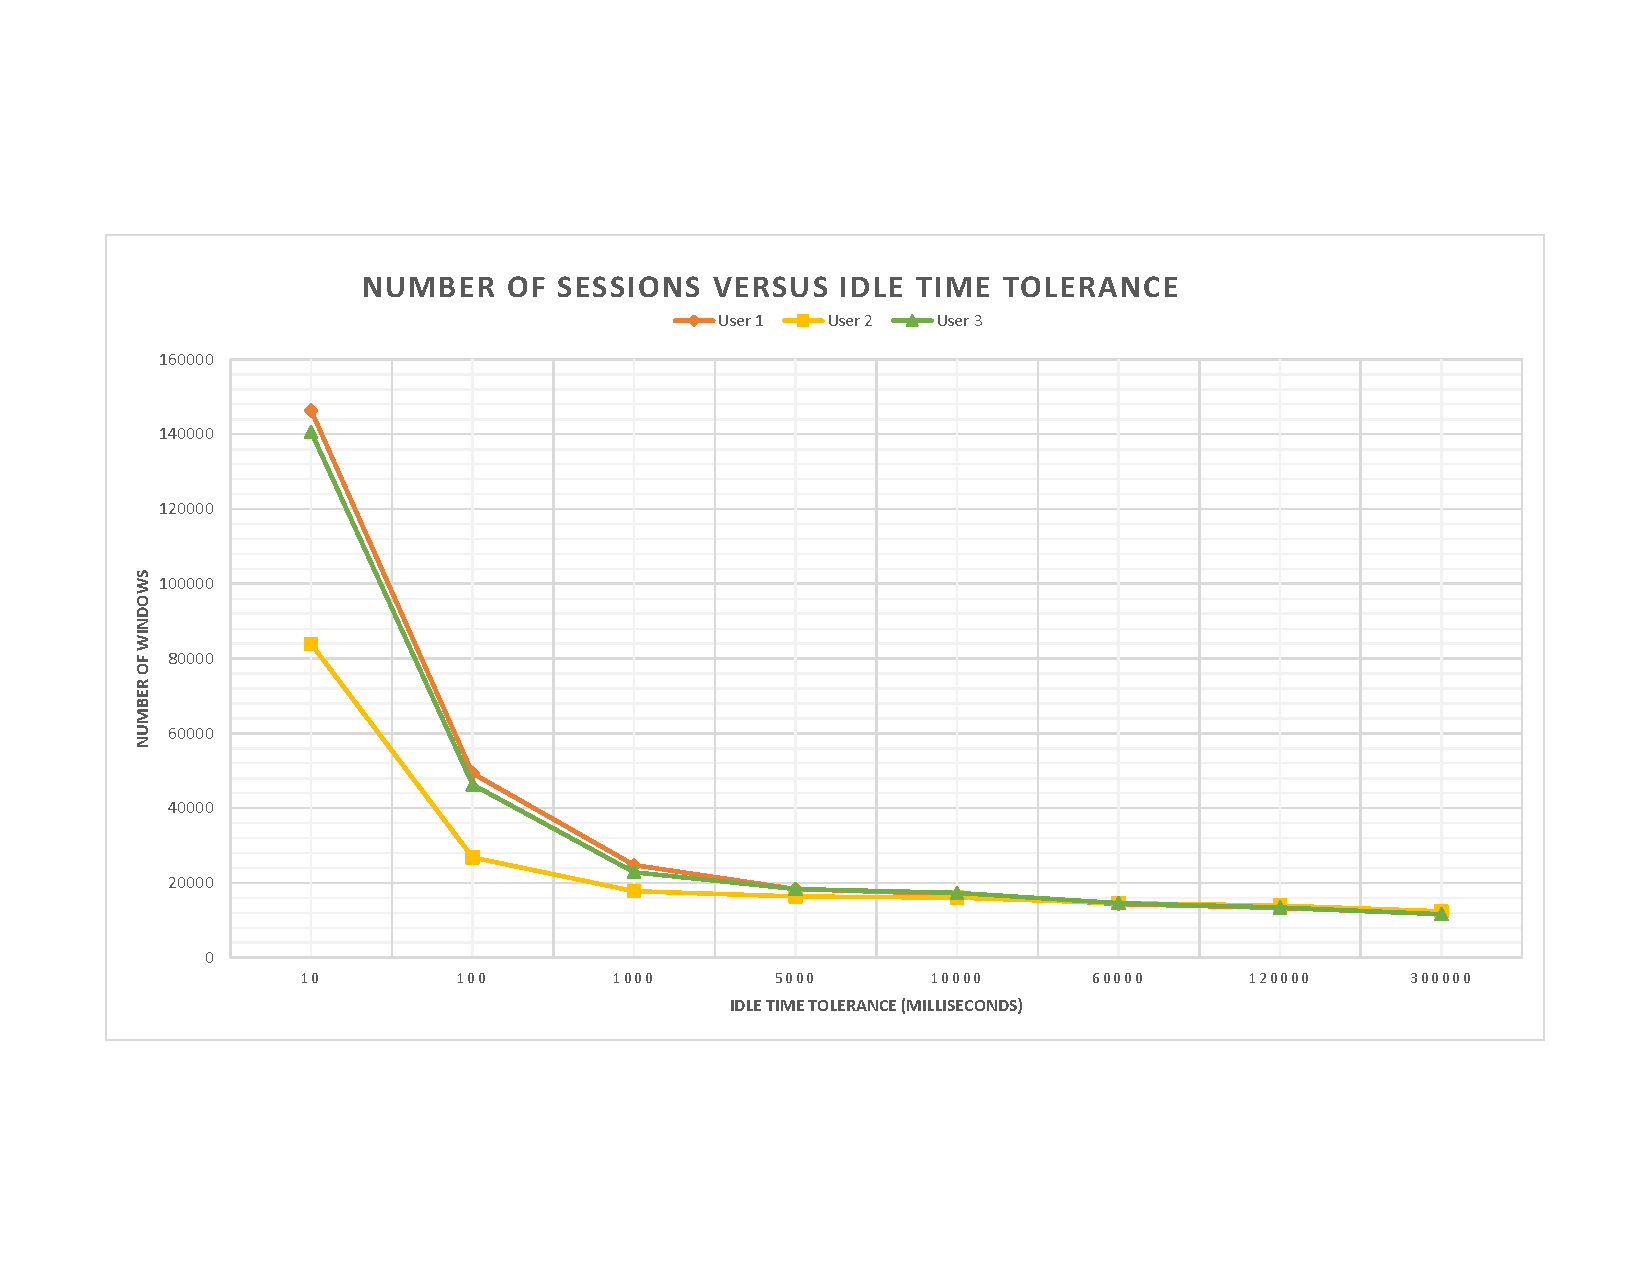
\includegraphics[width=0.5\textwidth]{graphics/IdleTimeTolerances}
    \caption{\todo{Regenerate}Number of user sessions generated with varying idle time tolerances}
    \label{fig:idletime}
\end{figure}

We incrementally iterate different idle time tolerances \textit{t} and look at the corresponding number of sessions that are obtained. The optimum value of \textit{t} is obtained by locating the knee or trade-off point. The non-optimum values of \textit{t} would require an unfavorably large change in one of the quantities to gain a small amount in the other. \cite{satopaa2011finding}
This method can implicitly adapt to workloads with different characteristics since the trade-off point is choosen by running through the actual query log.

%In our framework, a \textit{database session} on a smartphone is a time period in which the user's activity makes the application issue sequential queries with a period of at most \textit{t} seconds between them.
%We identify the approximate the time \textit{t} for each user to find what constitutes of a session for each user.
% Large values of \textit{t} would create sessions which span longer amounts of time. These bloated sessions would capture multiple tasks which would reduce the granuarity of subsequent processing. On the other hand, very small values of \textit{t} would create very small sessions which span minuscule amounts of time and contain very less queries. Such tiny sessions might not capture complete tasks.
%We incrementally iterate different idle time tolerances \textit{t}, and determine the ideal \textit{t} when incrementing it starts not to affect the number of sessions identified.


%We harvest the features extracted for each query in a session, and create a bag of features.
%We measure the behavior difference between sessions with Jensen-Shannon divergence~\cite{fuglede2004jensen} which compares two given probability distributions.
%Therefore, we are able to determine distinctive session characteristics, as well as repeating ones.

\begin{algorithm}[h]
 \caption{Euclid’s algorithm}
 \begin{algorithmic}[1]
   \Require
   	\Statex $a \ge 0$, $b \ge 0$
   \Ensure
   	\Statex the gcd of $a$ and $b$
   \Function{gcd}{$x, y$} \Comment{Where $a \ge 0$, $b \ge 0$}
     \If {$b = 0$}
       \Return $a$
     \Else $\;$
       \Return \Call{gcd}{$b, a \bmod b$}
     \EndIf
   \EndFunction
 \end{algorithmic}
\end{algorithm}

% Soikkeli \textit{et al.}~\cite{soikkeli2011diversity} say that even considering the time between launch and close of an application is not a reliable notion of an application usage session. Applications running in the foreground are visible to the user. Applications which are running in background are not visible to user even though he might have launched them before. 
% An individual session now consists of two parameters: a start time and an end time. 
% Two user sessions can be back to back or might have an idle time in between them. User sessions for a single application can be modeled as a time-wise closely-spaced series of queries issued to the smartphone database. A threshold value \textit{T} is defined for the idle time between two queries. If the idle time is less than or equal compared to \textit{T}, the queries belongs belong to the same user session. This session would contain a chronologically ordered subset of queries issued to the smartphone database. 


